\documentclass[a4paper,12pt]{article}
\usepackage{graphicx}
\usepackage{titlesec}
\usepackage[utf8]{inputenc}
\usepackage{xcolor}
\usepackage{fancyhdr}
\usepackage{lipsum}
\usepackage{caption}
\usepackage{tabularx,ragged2e}

\newlength\mylength
\settowidth{\mylength}{Oven Temperature: $160^{\circ}$C}
\addtolength\mylength{-2\tabcolsep}
\addtolength\mylength{-\arrayrulewidth}
\setlength\mylength{\dimexpr\mylength/2\relax}
\newcolumntype{P}[1]{>{\centering\arraybackslash}p{#1}}
% Width of column 1 is a residual
\newcolumntype{Y}{>{\RaggedRight}X}
% Handy shortcut macro
\newcommand\mc[1]{\multicolumn{2}{c|}{#1}}

\renewcommand{\headrulewidth}{0pt}
\fancyhead[C]{}
\fancyhead[C]{
	
\includegraphics[width=4cm]{metu}
}
\pagestyle{plain}
\usepackage[symbol*]{footmisc}
\DefineFNsymbolsTM{myfnsymbols}{% def. from footmisc.sty "bringhurst" symbols
	\textasteriskcentered *
	\textdagger    \dagger
	\textdaggerdbl \ddagger
	\textsection   \mathsection
	\textbardbl    \|%
	\textparagraph \mathparagraph
}%
\setfnsymbol{myfnsymbols}
%opening
\title{Middle East Technical University\\Department of Physics\\\textbf{PHYS307 Applied Modern Physics}}
\author{Oğuzhan ÖZCAN\\1852334}
\date{}
\clearpage
\thispagestyle{empty}
\providecommand{\groupmember}[1]{\textbf{Group Members:} }
\providecommand{\expdate}[1]{\textbf{Experiment Date:} }
\providecommand{\repdate}[1]{\textbf{Report Submit Date:} }
\providecommand{\expname}[1]{\textbf{Exp. MP-AS Franck-Hertz Experiment\footnote{Nobel Prize in Physics, 1925}} }


\usepackage[a4paper,%
left=0.5in,right=0.5in,top=0.35in,bottom=0.8in,%
footskip=.25in]{geometry}
%\topmargin -4.5cm
%\oddsidemargin 0.2cm
%\textwidth 16cm %
%\textheight 21cm%
%\footskip 1.0cm%




\begin{document}
\pagenumbering{gobble}
\maketitle

\thispagestyle{fancy}

%%%%%%%%%%%%%%%%%%%%%%%%%%%%%%%%%%%%%%%%%%%%%%%%%%%%%
\noindent\rule{18.4cm}{0.8pt}
\begin{center}
	\expname{arg1}{}
\end{center}
\groupmember{arg1}{Cem MADEN, İrem KÜL, Deniz AKYÜREK}\\
\expdate{November 6, 2015}{November 6, 2015}\\
\repdate{arg1}{November 13, 2015}\\
\noindent\rule{18.4cm}{0.8pt}\\\\
%%%%%%%%%%%%%%%%%%%%%%%%%%%%%%%%%%%%%%%%%%%%%%%%%%%%%
\begin{table}[h!]
	\setlength\tabcolsep{4pt}
	\caption{Data for different filament and collector voltages at instant oven temperature} \label{my-label}
	\begin{tabularx}{\textwidth}{|Y|*{4}{P{\mylength}|}}
		\hline
		& \mc{Filament Voltage: 6.0 V} & \mc{Filament Voltage: 6.0 V} \\
		& \mc{Collector Voltage: 2.0 V} & \mc{Collector Voltage: 2.0 V} \\
		& \mc{Oven Temperature: $160^{\circ}$C} & \mc{Oven Temperature: $160^{\circ}$C} \\
		\hline
		Voltage at first minimum\slash maximum [V] & 0 & 2.2 & 0 & 2.2 \\ \hline
		Voltage at second minimum\slash maximum [V] & 4.6 & 5.2 & 4.3 & 7.2 \\ 
		\hline
		Voltage at third minimum\slash maximum [V] & 9.6 & 12.4 & - & - \\ \hline
		Voltage difference between first and second minima\slash maxima [V] & 4.6 & 3.0 & 4.3 & 5.0 \\ 
		\hline
		Voltage difference between second and third minima\slash maxima [V] & 5.0 & 7.2 & - & - \\ 
		\hline
		Mean of Voltage difference between the minima\slash maxima [V] & 4.8 & 5.1 & 4.3 & 5.0 \\ 
		\hline
	\end{tabularx}
\end{table}

\textbf{Data \& Results}\\
Mean and the standard deviation of the first excited energy level: \textbf{4.8$\pm$0.2 eV}\\
Calculation of standard deviation $\sigma$ as follows:
\begin{equation}
(4.6-4.8)^2=-0.2^2=0.04
\end{equation}
\begin{equation}
(5.0-4.8)^2=0.2^2=0.04
\end{equation}
\begin{equation}
\frac{0.04+0.04}{2}=0.04
\end{equation}
Therefore standard deviation $\sigma$ in this case
\begin{equation}
\sigma=\sqrt{0.04}=0.2
\end{equation}
Accepted value of the first excited energy level: \textbf{4.9 eV}\\
Contact Potential difference between the anode and the cathode: \textbf{4.0 V} and \textbf{6.0 V}\\\\\\
\textbf{1. What are the advantages and disadvantages of the method used in this experiment by comparing with the optical methods?}\\\\
Optical methods of determining the excitation states suggested by Niels Henrik David Bohr. One important postulates of Bohr's is that radiation is only emitted when an atom makes transitions between
stationary states:
\begin{equation}
E_{ph}=E_{m}-E_{n}
\end{equation}
Main disadvantage of optical method is that atoms do not absorb at all the same wavelengths
that it emits. Isolated atoms are normally found in the ground state - excited
states live for very short time periods ($\approx $ 1 ns) before decaying to the ground
state. The absorption spectrum therefore contains only transitions from the
ground state (\textit{n = 1}). To observe transitions from the first excited state
(\textit{n = 2}) would require a significant number of atoms to occupy this state
initially. Another disadvantage when try to determine excited states of atoms we need to use their thermal energies this states that  to excite an atom to the first excited state from the ground
state requires temperature that satisfies [1]
\begin{equation}
k_{B}T = E_{2} - E{1} = 10.2 eV
\end{equation}
which gives a temperature 
\begin{equation}
T=\frac{(10.2eV)(1.6\times 10^{-19}J/eV)}{1.38\times 10^{-23}J/K}\approx 1.2\times 10^{5}K
\end{equation}
which much larger than the room temperature (surface of the sun has temperature of $6.3\times 10^{3}$ K.). If we need to provide a disadvantage of Franck-Hertz experiment that may be the experiment only must be performed by monoatomic gas like mercury (Hg), neon (Ne) and argon (Ar).\\\\\\
\textbf{Discussion and Conclusion}\\\\
In this we carried out a crucial experiment in Physics which is done by James Franck and Gustav Hertz in 1914. This experiment is proof of Bohr's Model. However, J. Franck and G. Hertz were not trying to test Bohr's model. As J. Franck admitted later, in fact, they were not even aware of Bohr's theory. They won their Nobel Prize 11 years later in 1925 because when they publish their paper \textit{Collision between Electrons and Mercury Vapor Molecules and the Ionization Potential of Such Molecules} there were some mistakes [2]. In the summary part of the paper, the fourth result claim that \textit{ionization potential of mercury is 4.9 volts.} However, this result is not quite correct because The mercury atoms are not being ionized by their collisions with electrons; they are simply being bumped upwards into an excited state [3]. Although J. Franck and G. Hertz made some mistakes in their work, Franck-Hertz Experiment can prove the Bohr's model. The deficiencies of Bohr model are as follows:\\\\
\textbullet  Cannot be applied to multi-electron atoms.\\
\textbullet Does not predict fine structure of atomic spectral lines.\\
\textbullet Does not provide a method to calculate relative intensities of spectral
lines.\\
\textbullet Predicts the wrong value of angular momentum for the electron in the
atom.\\
\textbullet Violates the Heisenberg uncertainty principle (although Bohr’s model
preceded this by more than a decade)\\\\
\newpage
In summary, in this experiment we studied the excitation state of mercury atom. We realized there are two different way to find excitation state of an atom: optical method and this experiment. While doing experiment, we had to set temperature at $\approx160^{\circ}$ C but we could not do that. That is why our results are not quite correct. Normally we can determine $n=5$ state but we reached to $n=3$ state. Therefore we can say that our experiment is nearly incomplete. Figure 1 shows this result.\\\\\\
\begin{figure}[h!]
\centering
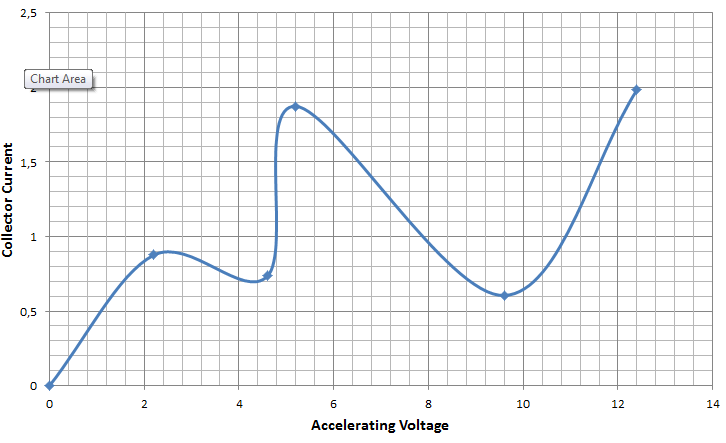
\includegraphics[width=0.85\linewidth, height=0.35\textheight]{Capture}
\caption{Collector Current $I_{c}$ versus Accelerating Voltage $V_{a}$}
\label{fig:Capture}
\end{figure}

\textbf{References}\\\\
$[1]$ A. Melissinos, \textit{Experiments in Modern Physics} (Academic
Press Inc., 1966) p.14.\\
$[2]$ J. Franck \& G. Hertz, \textit{Verhand. Deut. Physik, Ges.,} 16 (1914), 457-467.\\
$[3]$ Mott and Massey, \textit{The theory of atomic collisions},
(Oxford University Press, 1971) p.185, 3rd ed.\\



















\end{document}
